% Results and Discussion section drafted from committed result artifacts.
% This file is a section fragment, not a standalone LaTeX document.

\section{Results and Discussion}
\label{sec:results_discussion}

\subsection{Main Quantization Results}
\label{subsec:main_quantization_results}

Table~\ref{tab:main_results} reports Top-1 accuracy on the CIFAR-10 test set, accuracy drop relative to FP32, activation reconstruction MSE, and logit MSE.

\begin{table*}[t]
\centering
\caption{Main results on CIFAR-10. Accuracy is evaluated on the CIFAR-10 test set. Activation MSE and logit MSE are used to characterize simulated quantization error.}
\label{tab:main_results}
\begin{tabular}{l c c l l c c c c}
\hline
\textbf{Method} & \textbf{W bits} & \textbf{A bits} & \textbf{Act. site} & \textbf{Act. granularity} & \textbf{Top-1 (\%)} & \textbf{Drop (pp)} & \textbf{Act. MSE} & \textbf{Logit MSE} \\
\hline
FP32 & 32 & 32 & none & none & 94.1300 & 0.0000 & 0.00000000 & 0.00000000 \\
INT8-MinMax & 8 & 8 & conv\_linear\_output & per\_tensor & 94.1100 & 0.0200 & 0.00005792 & 0.00910544 \\
INT4-MinMax & 4 & 4 & post\_relu & per\_tensor\_per\_relu\_module & 88.2000 & 5.9300 & 0.00273660 & 1.84912006 \\
INT4-P99.9 & 4 & 4 & post\_relu & per\_tensor\_per\_relu\_module & 92.9700 & 1.1600 & 0.00035606 & 0.46350010 \\
INT4-MSE-Selected & 4 & 4 & post\_relu & per\_tensor\_per\_relu\_module & 92.8600 & 1.2700 & 0.00034846 & 0.41728575 \\
\hline
\end{tabular}
\end{table*}

INT8-MinMax remains close to FP32, with 94.1100\% Top-1 accuracy compared with 94.1300\% for FP32. In contrast, INT4-MinMax drops to 88.2000\%, a 5.9300 percentage-point decrease. In this evaluated CIFAR-10 ResNet-18 run, both implemented clipping variants alleviate this degradation: INT4-P99.9 reaches 92.9700\%, while INT4-MSE-Selected reaches 92.8600\%. Compared with INT4-MinMax, INT4-MSE-Selected improves Top-1 accuracy and reduces the accuracy drop from 5.9300 to 1.2700 percentage points.

The result should be interpreted conservatively. INT4-MSE-Selected improves over INT4-MinMax and reduces reconstruction error, but it does not exceed the fixed INT4-P99.9 baseline in Top-1 accuracy in this run. Therefore, the experiment supports mitigation of INT4-MinMax degradation in the implemented setting, not a claim that the studied method is uniformly better than fixed percentile clipping.

\subsection{Error Metric Analysis}
\label{subsec:error_metric_analysis}

\begin{figure}[t]
\centering
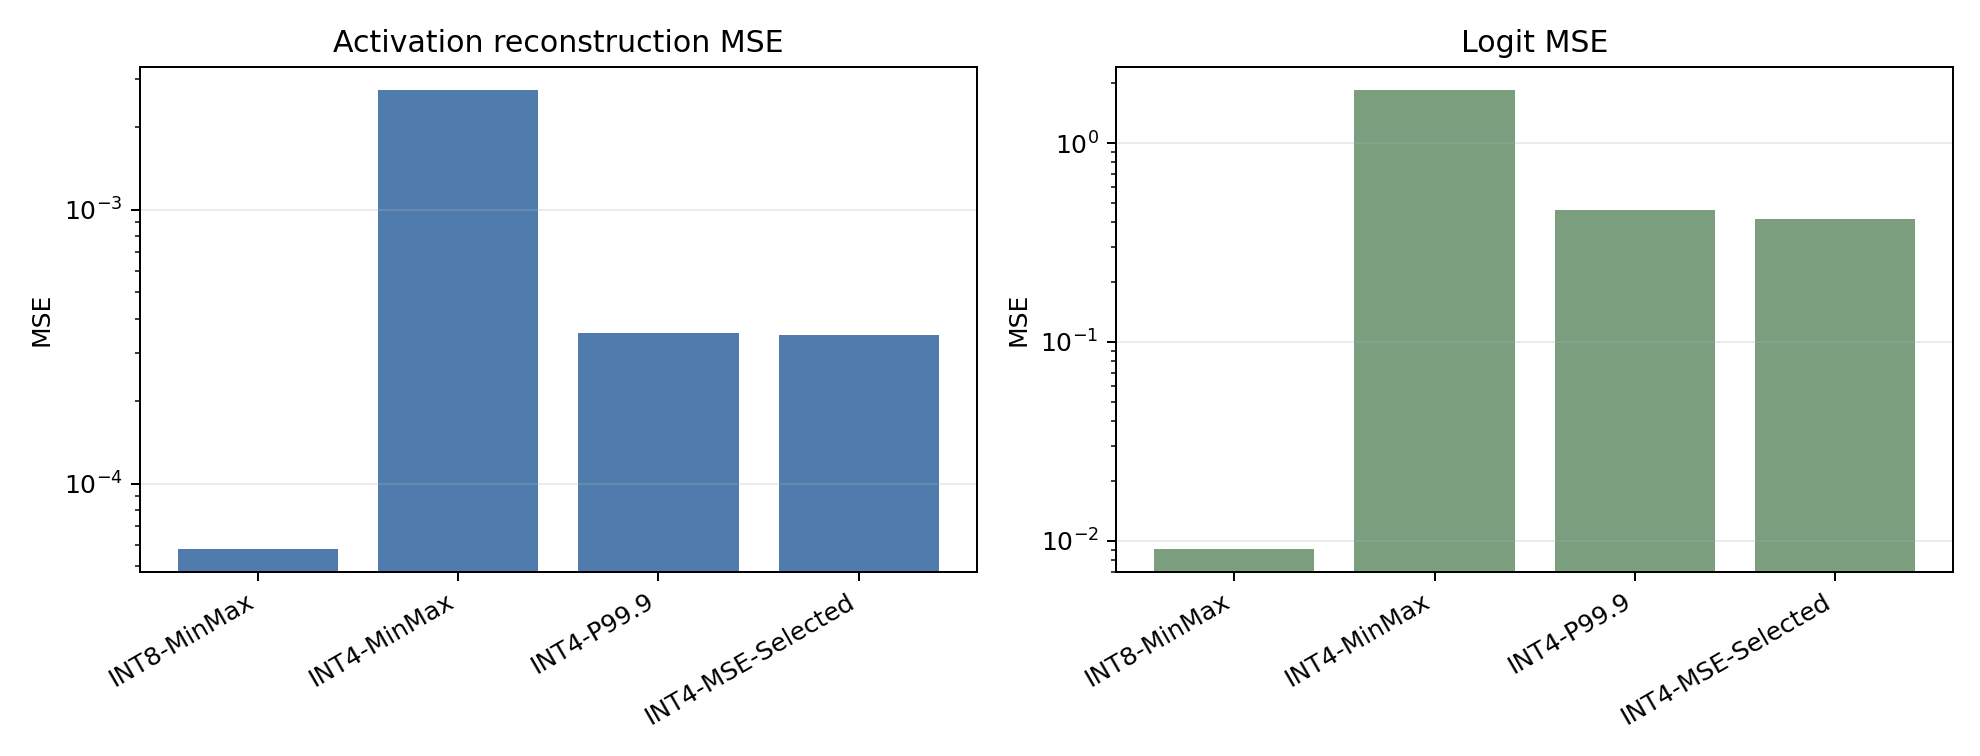
\includegraphics[width=\linewidth]{outputs/figures/error_metrics.png}
\caption{Activation reconstruction MSE and logit MSE of the quantized methods. The figure visualizes the error metrics reported in Table~\ref{tab:main_results}.}
\label{fig:error_metrics}
\end{figure}

Compared with INT4-MinMax, INT4-MSE-Selected reduces activation reconstruction MSE from 0.00273660 to 0.00034846 and logit MSE from 1.84912006 to 0.41728575. It also has slightly lower activation MSE and logit MSE than INT4-P99.9, although this lower reconstruction error does not translate into the highest Top-1 accuracy. In this setting, this mismatch suggests that calibration reconstruction MSE is useful for analyzing simulated quantization behavior but is not a complete substitute for test-set accuracy.

\subsection{Activation Distribution Interpretation}
\label{subsec:activation_distribution_interpretation}

Although this work does not report a separate activation histogram figure, the activation distribution perspective provides a plausible qualitative explanation for why clipping may help low-bit activation quantization in this setting: rare large post-ReLU values can stretch the MinMax range, while high-percentile or MSE-selected clipping trades limited saturation for lower rounding error on common activation values. The discussion is therefore limited to this qualitative interpretation rather than a layer-specific numerical claim.

\subsection{Layer-wise Activation MSE}
\label{subsec:layerwise_activation_mse}

\begin{figure}[t]
\centering
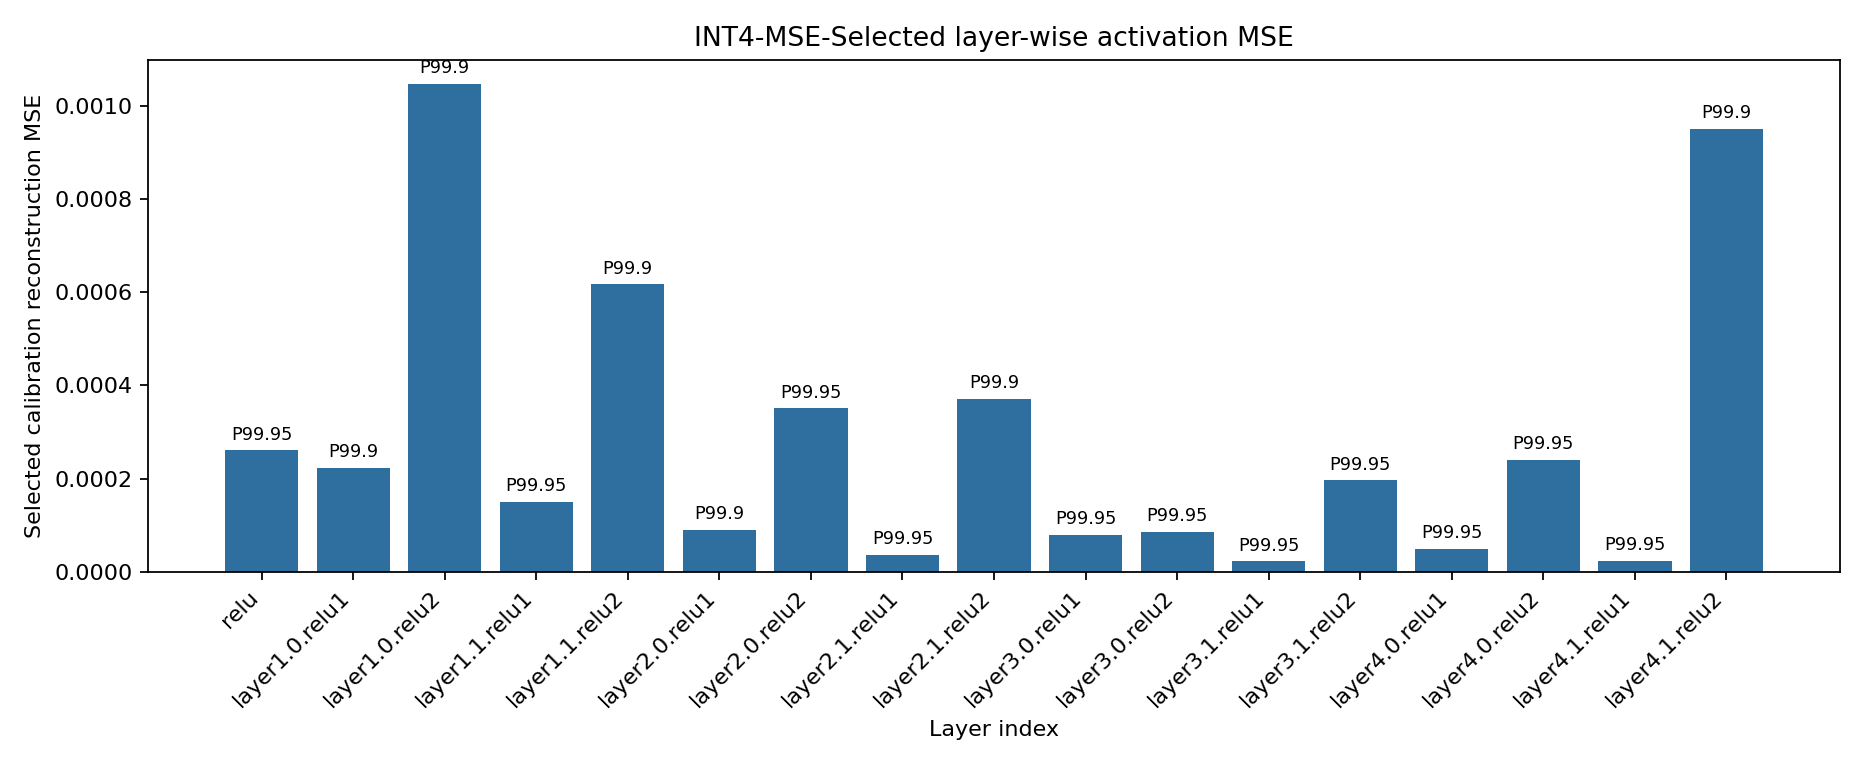
\includegraphics[width=\linewidth]{outputs/figures/layerwise_mse.png}
\caption{Layer-wise selected activation reconstruction MSE for INT4-MSE-Selected. The annotations indicate the selected percentile for each observed post-ReLU activation site.}
\label{fig:layerwise_mse}
\end{figure}

As visualized in Fig.~\ref{fig:layerwise_mse}, selected percentiles and reconstruction errors vary across observed post-ReLU activation sites. This confirms that the implemented calibration rule is applied layer-wise within the predefined candidate set. The result should not be interpreted as continuous globally optimal clipping, because the search is restricted to \(\{99.0,99.5,99.9,99.95,100.0\}\).

\subsection{Discussion and Limitations}
\label{subsec:results_limitations}

In this controlled CIFAR-10 ResNet-18 setting and for the implemented baselines, activation clipping reduces the degradation of simulated INT4 PTQ relative to a plain MinMax baseline. However, the current result is based on one dataset, one model, one random seed, and one configuration. No multi-seed study, calibration-size sweep, multi-architecture evaluation, or QAT comparison is reported. The implementation is simulated PTQ with fake quantization and dequantization; no real INT4 inference kernel, hardware latency, throughput, energy measurement, or deployment speedup is reported. We also do not compare against stronger reconstruction-based PTQ methods such as AdaRound or BRECQ, so the results should be viewed as a controlled comparison among the implemented baselines rather than a comprehensive PTQ benchmark.
